\documentclass{beamer}
\usepackage{movie15}
\usepackage{multirow}
\usepackage{amsmath}
\usepackage{amsthm,amsthm}
\usepackage{amssymb}
\usepackage{multicol}

\definecolor{lightblue}{rgb}{0,0.7,0.7}

\global\long\def\ev{\mathbb{E}}
\usetheme{metropolis}           % Use metropolis theme
\title{ A Kernel Test of Goodness of Fit}
\date{\today}
\author{Kacper Chwialkowski, Heiko Strathmann, Arthur Gretton}
\institute{Gatsby Unit and CS Department, UCL}
\titlegraphic{
    %\includegraphics[width=2cm]{csml_logo_vector2.pdf}\hspace*{4.75cm}~%
   \includegraphics[width=2cm]{./img/csml_logo_vector2.pdf}
}

\definecolor{mg}{rgb}{0,0.44,0}


\definecolor{1}{rgb}{ 0.9000,0.4909,0}
\definecolor{2}{rgb}{ 0.8182 ,   0.9000,         0}
\definecolor{3}{rgb}{ 0.3273,    0.9000    ,     0}
\definecolor{4}{rgb}{    0  ,  0.9000 ,   0.1636}
\definecolor{5}{rgb}{   0  ,  0.9000  ,  0.6545}
\definecolor{6}{rgb}{   0  ,  0.6545   , 0.9000}
\definecolor{7}{rgb}{  0  ,  0.1636 ,   0.9000}
\definecolor{8}{rgb}{ 0.3273  ,       0  ,  0.9000}
\definecolor{9}{rgb}{ 0.8182  ,       0  ,  0.9000}
\definecolor{10}{rgb}{  0.9000  ,       0  ,  0.4909}



\newtheorem{thm}{Theorem}



\begin{document}
\frame{\titlepage}
  \setbeamercolor{background canvas}{bg=white}
 \begin{frame}{Motivating example: testing output of approximate MCMC}
 \begin{center}
   Approximate MCMC: tradeoff between bias and computation\\ (e.g. {\em Austerity in MCMC Land} \cite{korattikara2013austerity})
   \end{center}
\begin{columns}
        \begin{column}{.7\textwidth}
   \includegraphics[width=\textwidth]{./img/sgld_trace_and_density.pdf} 
        \end{column}
        \begin{column}{.3\textwidth}
$\theta_{1}\sim{\cal N}(0,10);\theta_{2}\sim{\cal N}(0,1)$\\
$ X_{i}\sim\frac{1}{2}{\cal N}(\theta_{1},4)+\frac{1}{2}{\cal N}(\theta_{1}+\theta_{2},4) $.
        \end{column}
\end{columns}
 \vspace{0.3cm}
\begin{center}
 {\large\emph{{\color{red} How to check if MCMC samples match target distribution?}}}
 \end{center}
 \end{frame}
 
 \begin{frame}{Maximum mean discrepancy: metric between ${ \color{red} p}$ and ${\color{lightblue} q}$ }
 \begin{center}
$MMD({\color{red} p},{ \color{blue} q},F) = \sup_{   \| {\color{mg}f} \|_F<1} [\ev_{{ \color{blue} q}}{\color{mg}f}- \ev_{{\color{red} p}}{\color{mg} f}]  $\\
\vspace{0.5cm}
 \includegraphics[width=0.6\textwidth]{./img/mmd.pdf} 
 \end{center}
 \begin{itemize}
  \item $F$ is an Reproducing Kernel Hilbert Space.
  \item ${\color{mg} f^*}$ is the function that attains the supremum.
 \end{itemize}

Can we compute $MMD$ when ${\color{blue} q}$ are MCMC samples, ${\color{red} p}$ is model?

\pause

 \vspace{0.1cm}
\begin{center}
 {\large\emph{ {\color{red} Problem:} don't have $\ev_{{\color{red} p}}{\color{mg} f}$ in closed form }}
 \end{center}
 
 \end{frame} 
 
 
 
 \begin{frame}{Main idea (by Stein)}
To get rid of $\ev_{ {\color{red} p} }f$  in $$ \sup_{    \| {\color{mg}f} \|_F<1} [\ev_{{ \color{blue} q}}{\color{mg}f}- \ev_{{\color{red} p}} {\color{mg}f}] $$we will use the cornerstone of modern ML

\pause
\textbf{Integration by parts}

%\pause 
%not the chain rule

%\pause
%I got you

%\pause 
%\begin{flushright}
%\small \textit{Kacper} 
%\end{flushright}



\end{frame} 

  \begin{frame}{Stein's trick in the RKHS}
%  \begin{center}
Consider the  class \large
$$G = \{ f'  +  \log' { \color{red} p} \cdot  f | f \in \mathcal{F} \}$$
\normalsize

\pause

Given $g\in G$, then (integration by parts)
\begin{align*}
\ev_{\color{red} p} g(X) &=
\ev_{\color{red} p} \left[ f'(X)  +  \log' {\color{red} p}(X) f(X) \right] \\
&= \int   f(x)' { \color{red} p}(x)   + f(x){\color{red} p}'(x) dx \\
&= \int_{-\infty}^{\infty} (f(x) {\color{red} p}(x) )'  dx \\
&= f(x) {\color{red} p}(x)  \big|_{x=-\infty}^{x=\infty} \\
&= 0
\end{align*}

\scriptsize
See  \cite{gorham2015measuring,OatGirCho15}.
\normalsize
%  \end{center}
 \end{frame} 
  
%%%%%%%%%%%%%%%%%%%%%%%%%%%%%%%%%%%%%%%%%%%%%%%%%%%%%%%%%%%%%%%%%%%%%%%%%%%%%%%%
  
 \begin{frame}{Maximum Stein Discrepancy }
Define the {\bf Stein operator}
\[
 T_{\color{red} p}f =  f'  +  \log' { \color{red} p} \cdot  f
\]

\pause
{\bf {\color{red} Maximum Stein Discrepancy (MSD)}}

\vspace{-0.5cm}

\begin{center}
 %\scalebox{0.8}{ $G = \{ f  +  \log' {\color{red} p} f | f \in F \}$}
 
\begin{align*}
MSD({\color{red} p},{ \color{blue} q},G) = \sup_{   \| {\color{mg} g} \|_\mathcal{F}<1} \ev_{{ \color{blue} q}} T_{\color{red} p} {\color{mg} g} - \ev_{{\color{red} p}} T_{\color{red} p} {\color{mg} g}  = \sup_{ \| {\color{mg} g} \|_\mathcal{F}<1} \ev_{{ \color{blue} q}} T_{\color{red} p} {\color{mg} g} 
\end{align*}
\pause \vspace{0.5cm}
 \includegraphics[width=0.8\textwidth]{./img/s1.pdf} 
 \end{center}

\vspace{-1cm}
   \scriptsize
    $G = \{ T_{\color{red} p}f | f \in \mathcal{F} \}$.
\normalsize
 \end{frame}

 %%%%%%%%%%%%%%%%%%%%%%%%%%%%%%%%%%%%%%%%%%%%%%%%%%%%%%%%%%%%%%%%%%%%%%%%%%%%%%%%
  
  
  \begin{frame}{Maximum Stein Discrepancy }
Define the {\bf Stein operator}
\[
 T_{\color{red} p}f =  f'  +  \log' { \color{red} p} \cdot  f
\]

{\bf {\color{red} Maximum Stein Discrepancy (MSD)}}

\vspace{-0.5cm}

\begin{center}
 %\scalebox{0.8}{ $G = \{ f  +  \log' {\color{red} p} f | f \in F \}$}
 
\begin{align*}
MSD({\color{red} p},{ \color{blue} q},G) = \sup_{   \| {\color{mg} g} \|_\mathcal{F}<1} \ev_{{ \color{blue} q}} T_{\color{red} p} {\color{mg} g} - \ev_{{\color{red} p}} T_{\color{red} p} {\color{mg} g}  = \sup_{ \| {\color{mg} g} \|_\mathcal{F}<1} \ev_{{ \color{blue} q}} T_{\color{red} p} {\color{mg} g} 
\end{align*}
     \vspace{0.5cm}
 \includegraphics[width=0.8\textwidth]{./img/s05.pdf} 
 \end{center}

\vspace{-1cm}
   \scriptsize
    $G = \{ T_{\color{red} p}f | f \in \mathcal{F} \}$.
\normalsize
 \end{frame}
 

%%%%%%%%%%%%%%%%%%%%%%%%%%%%%%%%%%%%%%%%%%%%%%%%%%%%%%%%%%%%%%%%%%%%%%%%%%%%%%%%


  \begin{frame}{Maximum Stein Discrepancy }
Define the {\bf Stein operator}
\[
 T_{\color{red} p}f =  f'  +  \log' { \color{red} p} \cdot  f
\]

{\bf {\color{red} Maximum Stein Discrepancy (MSD)}}

\vspace{-0.5cm}

\begin{center}
 %\scalebox{0.8}{ $G = \{ f  +  \log' {\color{red} p} f | f \in F \}$}
 
\begin{align*}
MSD({\color{red} p},{ \color{blue} q},G) = \sup_{   \| {\color{mg} g} \|_\mathcal{F}<1} \ev_{{ \color{blue} q}} T_{\color{red} p} {\color{mg} g} - \ev_{{\color{red} p}} T_{\color{red} p} {\color{mg} g}  = \sup_{ \| {\color{mg} g} \|_\mathcal{F}<1} \ev_{{ \color{blue} q}} T_{\color{red} p} {\color{mg} g} 
\end{align*}
     \vspace{0.5cm}
 \includegraphics[width=0.8\textwidth]{./img/s01.pdf} 
 \end{center}

\vspace{-1cm}
   \scriptsize
    $G = \{ T_{\color{red} p}f | f \in \mathcal{F} \}$.
\normalsize
 \end{frame}
 
%%%%%%%%%%%%%%%%%%%%%%%%%%%%%%%%%%%%%%%%%%%%%%%%%%%%%%%%%%%%%%%%%%%%%%%%%%%%%%%%

   \begin{frame}{Maximum Stein Discrepancy }
Define the {\bf Stein operator}
\[
 T_{\color{red} p}f =  f'  +  \log' { \color{red} p} \cdot  f
\]

{\bf {\color{red} Maximum Stein Discrepancy (MSD)}}

\vspace{-0.5cm}

\begin{center}
 %\scalebox{0.8}{ $G = \{ f  +  \log' {\color{red} p} f | f \in F \}$}
 
\begin{align*}
MSD({\color{red} p},{ \color{blue} q},G) = \sup_{   \| {\color{mg} g} \|_\mathcal{F}<1} \ev_{{ \color{blue} q}} T_{\color{red} p} {\color{mg} g} - \ev_{{\color{red} p}} T_{\color{red} p} {\color{mg} g}  = \sup_{ \| {\color{mg} g} \|_\mathcal{F}<1} \ev_{{ \color{blue} q}} T_{\color{red} p} {\color{mg} g} 
\end{align*}
     \vspace{0.5cm}
 \includegraphics[width=0.8\textwidth]{./img/s0.pdf} 
 \end{center}

\vspace{-1cm}
   \scriptsize
    $G = \{ T_{\color{red} p}f | f \in \mathcal{F} \}$.
\normalsize
 \end{frame}
 
 
 %%%%%%%%%%%%%%%%%%%%%%%%%%%%%%%%%%%%%%%%%%%%%%%%%%%%%%%%%%%%%%%%%%%%%%%%%%%%%%%%
 
\begin{frame}{Maximum Stein Discrepancy has simple closed-form expression}

Closed-form expression for MSD: given $Z,Z'  \sim { \color{blue} q}$, then

%\underset{\mathrm{i.i.d.}}{\sim}

\Large
\[MSD({\color{red} p},{ \color{blue} q},G) = \ev_{{ \color{blue} q}} h_{{\color{red} p}}(Z,Z')\]
\normalsize
where
  \begin{align*}
h_{{\color{red} p}}(x,y) & := \partial_{x} \log {\color{red} p}(x) \partial_{x} \log {\color{red} p}(y) k(x,y)\\
 & \quad+\partial_{y} \log {\color{red} p}(y) \partial_{x}  k(x,y)\\
 & \quad+\partial_{x} \log {\color{red} p}(x) \partial_{y}k(x,y)\\
 & \quad+\partial_{x} \partial_{y} k(x,y).
\end{align*}
and $k$ is RKHS kernel for $F$



\begin{center}
 {\large\emph{  Only depends on kernel and $\partial_{x} \log {\color{red} p}(x)$. \\ Do not need
to normalize {\color{red} p}, or sample from it.   }}
 \end{center}


%  \scriptsize
%  Condition: $\ev_{{ \color{blue} q}} h_{{\color{red} p}}(Z,Z)<\infty$
%  \normalsize
  
\end{frame}

 %%%%%%%%%%%%%%%%%%%%%%%%%%%%%%%%%%%%%%%%%%%%%%%%%%%%%%%%%%%%%%%%%%%%%%%%%%%%%%%%


\begin{frame}{Maximum Stein Discrepancy zero $\iff$ ${ \color{red} p} =  {\color{lightblue} q}$}

%Let ${ \color{blue} q},{\color{red} p}$ be probability measures and $Z\sim { \color{blue} q}$. 
\begin{thm}
  If the kernel $k$ is $C_0$-universal, $\ev_{{ \color{blue} q}} h_{{ \color{blue} q}}(Z,Z)<\infty$ and\\
  $\ev_{{ \color{blue} q}} \left( \log' \frac{{\color{red} p}(Z)}{{ \color{blue} q}(Z)} \right)^{2}<\infty$
 then
\begin{center}
\large
  $MSD({\color{red} p},{ \color{blue} q},G) =0$ if and only if ${\color{red} p}={ \color{blue} q}$.
\normalsize
\end{center}
\end{thm}

\vspace{10mm}
\footnotesize{
Kernel is $C_0$-universal if  $f \to \int_X f(x) k(x,\cdot) d\mu(x)$ if is injective for all probability measures $\mu$ and all  $f \in L^p(X,\mu)$, where  $p \in [1,\infty] $. 

The assumption $\ev_{{ \color{blue} q}} \left(\log' \frac{{\color{red} p}(Z)}{{ \color{blue} q}(Z)}\right)^{2}<\infty$ states that difference between scores $\log' \color{red} p$ and $\log' \color{blue} q$  is square integrable. 
}

\end{frame} 

 %%%%%%%%%%%%%%%%%%%%%%%%%%%%%%%%%%%%%%%%%%%%%%%%%%%%%%%%%%%%%%%%%%%%%%%%%%%%%%%%

 
 \begin{frame}{Empirical estimate of MSD: $V$-statistic}

Empirical estimate  of $\ev_{\color{blue} q} h_{\color{red} p}(Z,Z')$ is
a {\em V-statistic}: 
\[
 V_n(h_{\color{red} p}) = \frac {1} {n^2} \sum_{i,j=1}^n h_{\color{red} p}(Z_i,Z_j),
\]
 $\{ Z_1 ,\ldots Z_t \ldots Z_n \}$ time series with marginal distrib.  {\color{blue} q}
   
\pause

%DEBUG: weak convergence discussion removed

%If ${\color{blue} q} =  {\color{red} p}$ then $ n V_n(h_{\color{red} p})$  converges weakly. 

%Otherwise, if ${\color{blue} q} \neq  {\color{red} p}$, statistic explodes, $P(n V_n(h_{\color{red} p}) <C) \to 0$.

\begin{center}
 {\large\emph{  What are ``typical'' values of  $\ev_{\color{blue} q} h_{\color{red} p}(Z,Z')$ when ${\color{red} p} = {\color{blue} q}$ ? }}
 \end{center}


 \end{frame}
 
 %%%%%%%%%%%%%%%%%%%%%%%%%%%%%%%%%%%%%%%%%%%%%%%%%%%%%%%%%%%%%%%%%%%%%%%%%%%%%%%%


 
  \begin{frame}{Distribution of statistic under null (${ \color{red} p} =  {\color{lightblue} q}$)}
To estimate quantiles of $ V_n(h_{\color{red} p})$ under the null  (when ${ \color{red} p} =  {\color{blue} q}$), we use {\bf wild bootstrap}
\[
 B_n(h_{\color{red} p}) = \frac {1} {n^2} \sum_{i,j=1}^n W_i W_j h_{\color{red} p}(X_i,X_j).
\]
  where $W_i$ are correlated zero mean RVs.
  
 \vspace{-0.3cm} 
\begin{columns}
        \begin{column}{.5\textwidth}
         $$
  Cov(W_i,W_j) = (1-2p_n)^{-|i-j|}
  $$
        \end{column}
        \begin{column}{.5\textwidth}
            \begin{figure}
            \vspace{-0.5cm}
           \includegraphics[width=0.7\textwidth, angle =0 ]{./img/W_graphicalModel.pdf} 
        \end{figure}
        \end{column}
    \end{columns}
%\vspace{-1cm}
    $p_n$ is  the probability of the change  and should be set to $o(n)$.
  \end{frame}

 \begin{frame}{Wild bootstrapping; small correlation }
\centering
 $$X_t = 0.1 X_{t-1} + \sqrt{1 - 0.1^2}\epsilon_t, \quad \epsilon_t \sim N(0,1)$$
 \includegraphics[width=0.9\textwidth]{./img/bootstrapWorks1.pdf}

 \end{frame}

 \begin{frame}{Wild bootstrapping, medium correlation}
\centering
 $$X_t = 0.4 X_{t-1} + \sqrt{1 - 0.4^2}\epsilon_t, \quad \epsilon_t \sim N(0,1)$$
 \includegraphics[width=0.9\textwidth]{./img/bootstrapWorks4.pdf}
\end{frame}

 \begin{frame}{Wild bootstrapping; huge correlation}
\centering
 $$X_t = 0.7 X_{t-1} + \sqrt{1 - 0.7^2}\epsilon_t, \quad \epsilon_t \sim N(0,1)$$
 \includegraphics[width=0.9\textwidth]{./img/bootstrapWorks7.pdf}
\end{frame}

 %%%%%%%%%%%%%%%%%%%%%%%%%%%%%%%%%%%%%%%%%%%%%%%%%%%%%%%%%%%%%%%%%%%%%%%%%%%%
 
 \iffalse

  \begin{frame}{Experiment 1: Student's t vs.~Normal}
\begin{columns}
        \begin{column}{.5\textwidth}
        \begin{figure}
           \includegraphics[width=\textwidth]{img/nt}   
        \end{figure}
        \end{column}
        \begin{column}{.5\textwidth}
            \begin{figure}
           \includegraphics[width=\textwidth]{img/sgld_student_opt} 
        \end{figure}
        \end{column}
    \end{columns}
Student's distributions was generated using MCMC.
\end{frame}

  \fi

 %%%%%%%%%%%%%%%%%%%%%%%%%%%%%%%%%%%%%%%%%%%%%%%%%%%%%%%%%%%%%%%%%%%%%%%%%%%%

 \begin{frame}{Experiment 1: Austerity in MCMC Land}
 \begin{center}
   Approximate MCMC: tradeoff between bias and computation\\ (e.g. {\em Austerity in MCMC Land} \cite{korattikara2013austerity})
   \end{center}
\begin{columns}
        \begin{column}{.7\textwidth}
   \includegraphics[width=\textwidth]{./img/sgld_trace_and_density.pdf} 
        \end{column}
        \begin{column}{.3\textwidth}
$\theta_{1}\sim{\cal N}(0,10);\theta_{2}\sim{\cal N}(0,1)$\\
$ X_{i}\sim\frac{1}{2}{\cal N}(\theta_{1},4)+\frac{1}{2}{\cal N}(\theta_{1}+\theta_{2},4) $.
        \end{column}
\end{columns}
 \end{frame}

 %%%%%%%%%%%%%%%%%%%%%%%%%%%%%%%%%%%%%%%%%%%%%%%%%%%%%%%%%%%%%%%%%%%%%%%%%%%%

\begin{frame}{Experiment 1: Austerity in MCMC Land}
 \begin{center}
   Approximate MCMC: tradeoff between bias and computation\\ (e.g. {\em Austerity in MCMC Land} \cite{korattikara2013austerity})
   \end{center}
\begin{columns}
        \begin{column}{.7\textwidth}
   \includegraphics[width=\textwidth]{img/Heiko1} 
        \end{column}
        \begin{column}{.3\textwidth}
$\theta_{1}\sim{\cal N}(0,10);\theta_{2}\sim{\cal N}(0,1)$\\
$ X_{i}\sim\frac{1}{2}{\cal N}(\theta_{1},4)+\frac{1}{2}{\cal N}(\theta_{1}+\theta_{2},4) $.
        \end{column}
\end{columns}
 \end{frame}
 

 

 %%%%%%%%%%%%%%%%%%%%%%%%%%%%%%%%%%%%%%%%%%%%%%%%%%%%%%%%%%%%%%%%%%%%%%%%%%%%
  
    \begin{frame}{Experiment 2: Statistical model criticism}
        \begin{figure}
           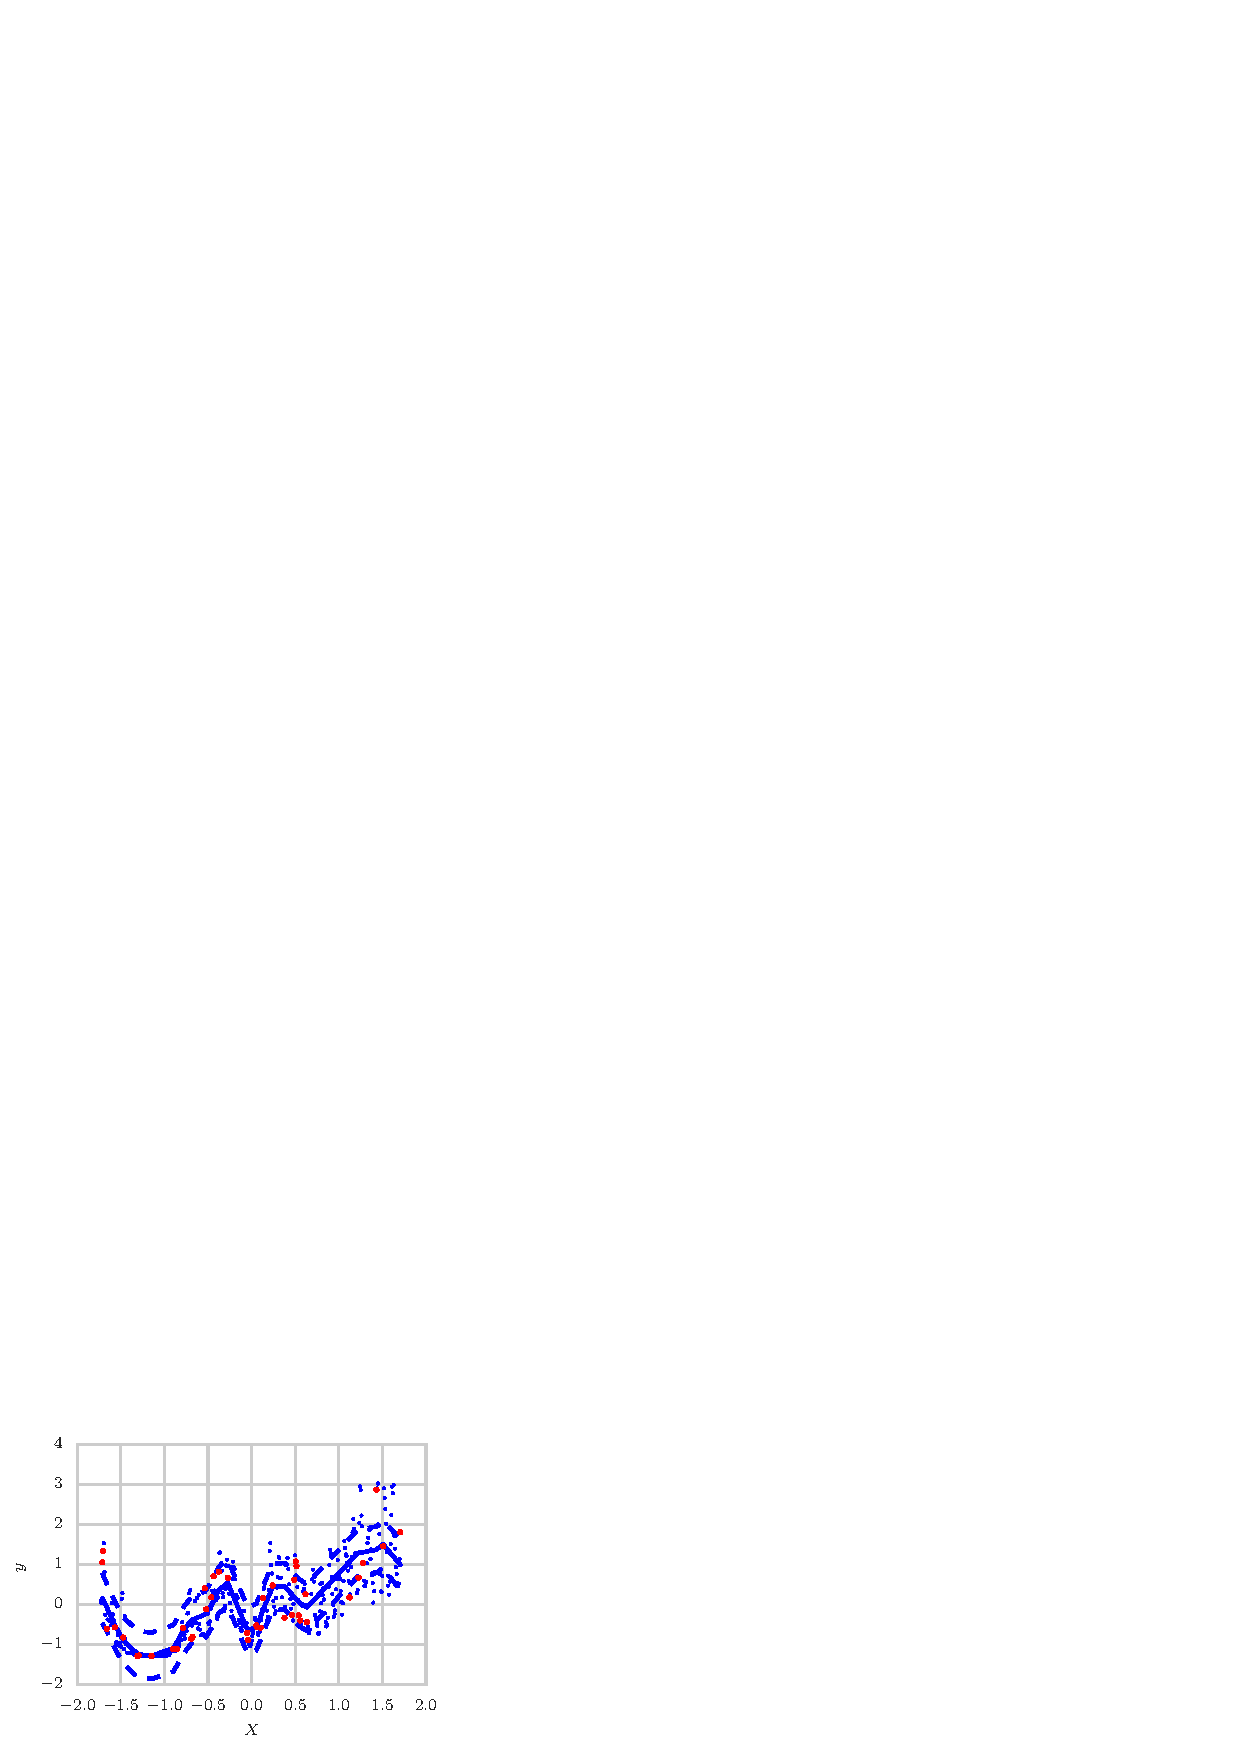
\includegraphics[width= 0.7\textwidth]{img/gp_regression_data_fit.pdf}  
        \end{figure}
We test the hypothesis that a Gaussian process {\color{red} model}, learned from \textbf{training data} $\star$, is a good fit for the {\color{blue} test data} \cite{lloyd2015statistical}.
  \end{frame}


   \begin{frame}{Experiment 2: Statistical model criticism}
        \begin{figure}
           \includegraphics[width=0.7\textwidth]{img/gp_regression_bootstrap_hist} 
        \end{figure}
We test the hypothesis that a Gaussian process {\color{red} model}, learned from \textbf{training data} $\star$, is a good fit for the {\color{blue} test data} \cite{lloyd2015statistical}.

   \end{frame}

   \begin{frame}{Questions?}
      \begin{figure}
\includegraphics[width=0.4\textwidth]{img/theKernel2} %vapnikBayes 0.7\textwidth
        \end{figure}   
   \end{frame}


   \begin{frame}{References}


\begin{minipage}{.9\linewidth}
{\tiny
%\begin{multicols}{2}
\setbeamertemplate{bibliography item}[text] 
\bibliographystyle{plain} 
\tiny
\bibliography{../biblio.bib} 
%\end{multicols}
} 
\end{minipage}
\end{frame}


\end{document}
